
%(BEGIN_QUESTION)
% Copyright 2012, Tony R. Kuphaldt, released under the Creative Commons Attribution License (v 1.0)
% This means you may do almost anything with this work of mine, so long as you give me proper credit

A {\it burner management system} (BMS) monitors the status of the flame at the base of this incinerator, to ensure fuel gas does not keep entering the combustion chamber unless there is an established fire to burn it:

$$\includegraphics[width=15.5cm]{i0004rx01.eps}$$

Explain the purpose of solenoid valve SV-115, identifying whether it is normally energized (NE) or normally de-energized (NDE).

\vskip 20pt \vbox{\hrule \hbox{\strut \vrule{} {\bf Suggestions for Socratic discussion} \vrule} \hrule}

\begin{itemize}
\item{} Is it possible to determine the ``normal'' energization statuses of solenoid valves SV-111, SV-112, and/or SV-113 from the information given in the diagram?  Explain why or why not.
\item{} Explain what may happen in this system if solenoid SV-111 were to fail.
\item{} Explain what may happen in this system if solenoid SV-103 were to fail.
\item{} Explain what may happen in this system if solenoid SV-113 were to fail.
\item{} Explain what may happen in this system if solenoid SV-102 were to fail.
\end{itemize}

\underbar{file i00866}
%(END_QUESTION)





%(BEGIN_ANSWER)


%(END_ANSWER)





%(BEGIN_NOTES)

SV-115 is normally energized, forcing FV-38 to go to its fail-safe (shut) position if ever the BMS detects a flame-out condition.

\vskip 10pt

We cannot determine the energization states of SV-111, SV-112, or SV-113 from this diagram because we do not see which state is passing versus blocking.












\vskip 20pt \vbox{\hrule \hbox{\strut \vrule{} {\bf Virtual Troubleshooting} \vrule} \hrule}

This question is a good candidate for a ``Virtual Troubleshooting'' exercise.  Presenting the diagram to students, you first imagine in your own mind a particular fault in the system.  Then, you present one or more symptoms of that fault (something noticeable by an operator or other user of the system).  Students then propose various diagnostic tests to perform on this system to identify the nature and location of the fault, as though they were technicians trying to troubleshoot the problem.  Your job is to tell them what the result(s) would be for each of the proposed diagnostic tests, documenting those results where all the students can see.

During and after the exercise, it is good to ask students follow-up questions such as:

\begin{itemize}
\item{} What does the result of the last diagnostic test tell you about the fault?
\item{} Suppose the results of the last diagnostic test were different.  What then would that result tell you about the fault?
\item{} Is the last diagnostic test the best one we could do?
\item{} What would be the ideal order of tests, to diagnose the problem in as few steps as possible?
\end{itemize}


%INDEX% Final Control Elements, valve: fail-safe solenoids
%INDEX% Process: incinerator (realistic P&ID shown)

%(END_NOTES)

